% !Tex root = Vorlage.tex
\newpage
\section{Execution}
A number of experiments have been conducted in order to evaluate the capabilities of empirical risk minimization (ERM) techniques for functional dependency discovery.
All rows containing missing values are dropped due to possible inconsistencies.

The measure chosen to compare imputation performance on columns containing continuous numeric values is the \emph{mean squared error} (MSE).
To compare classification performance, the F1-measure is chosen.

\subsection{FD Imputer}
FD Imputer is run for every FD found on a train subset of Adult and Nursery, respectively.
Figure~\ref{fig:f1_fd_adult} shows the performance of FD Imputer on columns containing classifiable data.
\begin{figure}[h]
     \centering
     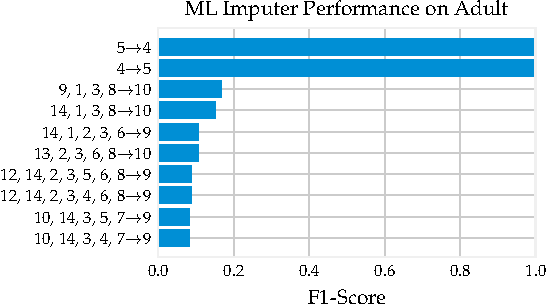
\includegraphics[width=.8\textwidth]{../figures/adult/f1_fd_imputer_adult.pdf}
     \caption{F1 score of the 10 most performant FDs when imputing values on a validation set.}
     \label{fig:f1_fd_adult}
 \end{figure}
The two top performing FDs have a perfect F1 score of 1 each.
An explanation for this can be found when analyzing the content of columns 4 and 5.
Column 4 contains information about the highest educational level achieved.

There are 16 different categories of educational level defined.
Each category is assigned an integer in a range from 0 to 15.
This integer is the content of column 5.
Thus, the relation between column 4 and column 5 can be modeled by a bijective function between the domains of each attribute.

Other FDs lead to F1 scores \(< 0.2\), yielding substantially worse results than the top two FDs.
It can be derived that only the two top-performing FDs hold in a general case.
If unseen data is added to the dataset, it can thus safely be assumed that these two FDs still hold.

\begin{table}[ht]
    \centering
    \begin{tabular}{lrrrrrr}
        \toprule
        & & & \multicolumn{4}{c}{Classification Performance} \\
        \cmidrule(lr{.25em}){4-7}
        Dataset & \# FDs & \# FDs\textsubscript{train} & F1\textsubscript{mean} & F1\textsubscript{max} & F1\textsubscript{min} & \# (F1 = 0) \\
        \midrule
        adult & 93 & 88 & 0.0669 & 1.0000 & 0.0000 & 10 \\
        nursery & 11 & 11 & 0.0000 & 0.0000 & 0.0000 & 10 \\
        \bottomrule
    \end{tabular}
    \caption{Performance of the FD Imputer.}\label{tab:fd-imputer-performance}
\end{table}

Table~\ref{tab:fd-imputer-performance} provides a summary of how FD Imputer performs.
The column ``\#~FDs'' indicates how many FDs were found on the complete dataset.
``\# FDS\textsubscript{train}'' contains the number of FDs that were detected on the train subset used for imputations.
``F1\textsubscript{mean}'', ``F1\textsubscript{max}'' and ``F1\textsubscript{min}'' indicate the arithmetic mean, maximal and minimal F1 score achieved on each dataset respectively.
The last column named ``\# (F1 = 0)'' provides the number of FDs that scored a F1 score of 0.

The results displayed in table~\ref{tab:fd-imputer-performance} show how strongly the FD Imputer's performance depends on the dataset considered.
On a dataset as normalized as nursery, FD Imputer cannot leverage FDs to impute unknown entries.

\subsection{ML Imputer}
ML Imputer is run with the same set of FDs as FD Imputer.
The 10 best performing FDs' F1 scores are displayed in figure~\ref{fig:f1_ml_adult}.
\begin{figure}[h]
     \centering
     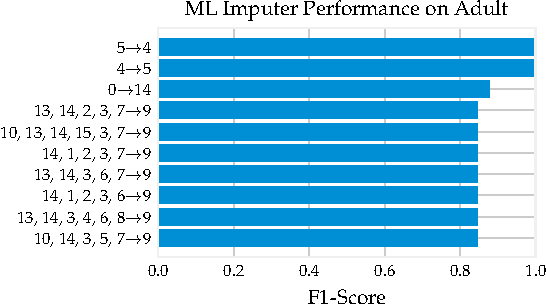
\includegraphics[width=.8\textwidth]{../figures/adult/f1_ml_imputer_adult.pdf}
     \caption{The figure compares the f1-score of the FD Imputer compared to the f1-score of the ML Imputer. Each point represents one FD.}
     \label{fig:f1_ml_adult}
 \end{figure}
The two top scoring FDs are the same for FD Imputer and ML Imputer.
The third most performant FD is a relation between row ID and nationality.
Since there is no appearent dependency between row ID and nationality, it is safe to assume that ML Imputer always guesses the most frequent nationality, US-American, for no matter what row ID.

This shows that ML Imputer is capable of learning Conditional Dependencies.

\begin{table}[ht]
    \centering
    \begin{tabular}{lrrrrrr}
        \toprule
        & & & \multicolumn{4}{c}{Classification Performance} \\
        \cmidrule(lr{.25em}){4-7}
        Dataset & \# FDs & \# FDs\textsubscript{train} & F1\textsubscript{mean} & F1\textsubscript{max} & F1\textsubscript{min} & \# (F1 = 0) \\
        \midrule
        adult & 93 & 88 & 0.7720 & 1.0000 & 0.0409 & 0 \\
        nursery & 11 & 11 & 0.4531 & 0.9915 & 0.1138 & 0 \\
        \bottomrule
    \end{tabular}
    \caption{Performance of the ML Imputer.}\label{tab:ml-imputer-performance}
\end{table}

\subsection{Overfitting the ML Imputer}

\subsection{Comparing ML Imputer with FD Imputer}
As discussed in the previous section, ML Imputer and FD imputer differ fundamentally in the way they function.
When comparing the two, metrics need to be computed bearing those differences in mind.

FD Imputer cannot approximate numerical values.
Due to the nature of the definition of a FD, Data is always assumed to be classifiable.
Meanwhile, ML Imputer is able to perform regression, predicting a continuous label for a given input with an uncertainty.

Naturally, this circumstance leads to a far superior performance of ML Imputer when imputing continuous labels.
FD Imputer usually doesn't find any values on the train set to impute with and cannot return a meaningful result.
Taking the above into account, rows that aren't imputed by FD Imputer are not considered when computing a performance measure on columns containing continuous values.

\begin{figure}[h]
     \centering
     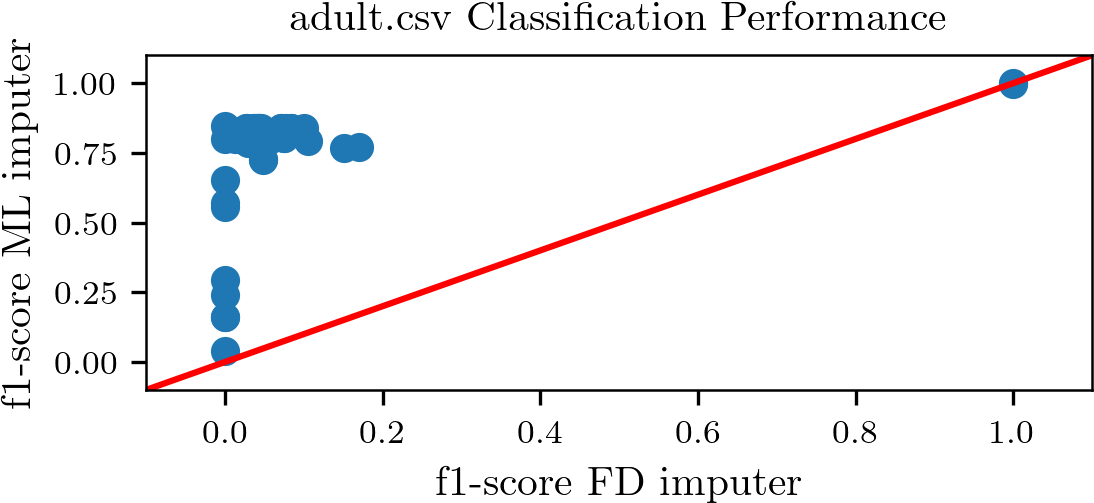
\includegraphics[width=.8\textwidth]{../figures/adult/f1_ml_fd_adult}
     \caption{The figure compares the f1-score of the FD Imputer compared to the f1-score of the ML Imputer. Each point represents one FD.}
     \label{fig:f1_ml_fd_adult}
 \end{figure}

Figure~\ref{fig:f1_ml_fd_adult} compares the F1-scores of both ML Imputer and FD Imputer on the Adult dataset.
One can observe that for most FDs, the ML Imputer performs better than the FD Imputer.
FD Imputer performance and ML Imputer performance seem to be proportional.
If the ML imputer's F1-score is lower than 0.7, the FD Imputer's F1-score for the same FD is 0.
However, for FD's where the ML Imputer scores are larger than 0.7, the FD Imputer scores better than 0.0.
Interestingly, there are two FDs for which the FD Imputer performs equally good or better than the ML Imputer.

The same comparison as
 \begin{figure}[h]
     \centering
     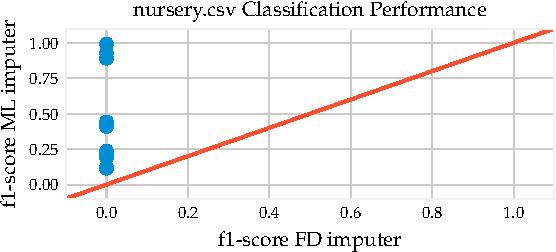
\includegraphics[width=.8\textwidth]{../figures/nursery/f1_ml_fd_nursery}
     \caption{Some ohter caption.}
     \label{fig:f1_ml_fd_nursery}
\end{figure}

\subsection{Classification Performance}
ML Imputer and FD Imputer were compared on two established Machine Learning datasets, Adult\footnote{\url{https://archive.ics.uci.edu/ml/datasets/adult}} and Nursery\footnote{\url{https://archive.ics.uci.edu/ml/datasets/nursery}}.
Adult's scheme is not normalized.
The table contains 70-something FDs.
In contrast to this, the Nursery dataset is strongly normalized.
It contains a mere 9 FDs, 8 of which are between the scheme's key and each attribute, respectively.

The complementary nature of these two datasets enables the observation of imputer performance in function of the degree of normalization.

\subsubsection{FD Imputer Performance}
\subsection{Begriffsdiskussion}
Lorem ipsum dolor sit amet, consetetur sadipscing elitr, sed diam nonumy eirmod
tempor invidunt ut labore et dolore magna aliquyam erat, sed diam voluptua. At
vero eos et accusam et justo duo dolores et ea rebum. Stet clita kasd gubergren,
no sea takimata sanctus est Lorem ipsum dolor sit amet.
